% sections/10_menu.tex -- Section 10, The Menu as a Whole (W2b). Plan: BLUEPRINT 2.10 and registry 8.8-8.10; Decisions 4, 7, 9;
% Overrides O1, O5, O8 (2-page budget including Figure 4). No displayed equations in this section (BLUEPRINT 3.2).
% Provenance abbreviations in "% src:" comments: T:x = paper/tables/x; T:age = welfare_age_dependence_mvpfv5.tex;
% T:prog = welfare_progressivity_mvpfv7.tex; T:med = welfare_medicare_mvpfv8.tex; T:tax = welfare_tax_mvpf_v8.tex;
% T:sav = welfare_savings_mvpf_v3.tex. Every cell quoted here is also listed in the header of figures/new/fig_wtpnet.tex.
\section{The Menu as a Whole}\label{sec:menu}

Sections~\ref{sec:claiming}--\ref{sec:other} evaluate the seven reform families one at a time; this section places every row side by side. Three columns are comparable across families: the MVPF, in dollars of welfare per dollar of net spending; the Net column, in percent of baseline government spending on the cohort; and the WTP column, in percent of consumption. The Indirect column is on a base that differs by family (\autoref{tab:conventions}) and is not compared across families, and the MVPF intervals of the saving subsidies, whose dollar conversion uses consumption from age 30 rather than from age 62, are kept out of the cross-family ordering (\autoref{sec:welfare}). % src: 12:611, 615, 620-622, 626 (bases); 12:632, 639 (consumption windows)

\subsection{Ranking within the menu}\label{subsec:ranking}

The sign of the Net column splits the menu in two. Net spending falls under AN1--AN3, AD1--AD5, AL1--AL9, and P1.1, and rises under every other row: P1.2--P3.9, L0--L9, both Medicare expansions, I1--I5, and K1--K3. % src: T:age:108-126 (Net -0.12 to -2.38); T:prog:115 (P1.1 Net -0.03), :116-158 (Net 0.09 to 1.29); T:med:113,116 (3.53, 3.19); T:tax:114-118 (0.69 to 3.46); T:sav:120-123 (0.08 to 1.34)
With the sign of the WTP column this gives three groups, the three populated quadrants of \autoref{fig:wtpnet}. AD1--AD5 and AL1--AL9 raise welfare and lower net spending: they are self-financing, their MVPF is infinite, and no finite lower bound exists because the program's own outlays fall as well (\autoref{subsec:returns}). P1.1 belongs to this group approximately: its net saving is 0.03 percent of baseline government spending, and its MVPF is the interval $[0.52,+\infty)$ of \eqref{eq:mvpflb}, whose lower end counts only the added retirement benefits. % src: T:age:112-126 (WTP > 0, Net < 0, Direct < 0); T:prog:115 (P1.1: Net -0.03, MVPF [0.52,+infty))
AN1--AN3 lower both welfare and net spending; their MVPF entries, 0.17, 0.16, and 0.18, are the values of reversing them. % src: T:age:108-110
Every remaining row raises both and has a finite MVPF.

Within this last group the MVPF orders the families as follows. First-bracket increases P1.2--P1.9 return 0.69 to 1.14 dollars of welfare per dollar of net spending; uniform increases L0--L9 return 0.30 to 0.61; second- and third-bracket increases P2.0--P3.9 return 0.29 to 0.56; income-tax reductions I1--I5 return 0.23 to 0.26. The Medicare expansions return 0.146 and 0.155, which with the reversal values of the NRA increases are the lowest finite values in the menu. % src: T:prog:116-123 (0.69-1.14), :149-158 (0.30-0.61), :126-146 (0.29-0.56); T:tax:114-118 (0.23-0.26); T:med:113,116 (0.146, 0.155); T:age:108-110 (0.16-0.18)
The saving subsidies have lower bounds of 0.96, 0.92, and 0.84, which divide the dollar welfare gain by the subsidy alone, and upper bounds of 20.37, 19.38, and 5.29, which divide it by the net cost under full taxation of the induced asset income. The lower bounds are the values used in the text, and because of the consumption window they are not ranked against the other families. % src: T:sav:120,122,123
In \autoref{fig:wtpnet}, by \eqref{eq:mvpfcolumns}, the MVPF within a family is proportional to the slope of the ray from the origin to a marker; the benefit-formula markers bend to the right from P2.5 on, which is the falling MVPF of \autoref{subsec:pmvpf}. % src: T:prog:131-146 (WTP 0.93-0.98 while Net 0.98-1.29)
The largest welfare gains in the menu, 3.6 percent of consumption under K3 and 2.09 under I5, come with increases in net spending of 1.34 and 3.46 percent, the latter close to the largest in the menu, 3.53 percent under Medicare Part A, whereas the gains of the claiming-schedule reforms, up to 0.80 percent under AL9, come with net savings. % src: T:sav:123 (K3: WTP 3.6, Net 1.34); T:tax:118 (I5: 2.09, 3.46); T:med:113 (Part A Net 3.53, the maximum of the Net column across the five tables); T:age:126 (AL9 WTP 0.80)

The ranking is a comparison within the menu under one accounting. It does not select a best reform, it says nothing about reforms outside the menu, and the MVPF enters it as a shadow price: a reform with positive net spending is worth undertaking when its MVPF exceeds the value placed on a dollar of public funds outside the cohort, and a self-financing reform at any such value \citep{hendren2020unified}. Appendix~\ref{app:netposition} states this formally. In the sense of \autoref{subsec:cohort}, the rows with negative Net contribute to closing the financing gap.

\subsection{What the participation columns say about the fiscal externality}\label{subsec:externality}

By \eqref{eq:decomp} and \eqref{eq:fm}, the fiscal effects beyond the mechanical outlay---the within-program behavioral change $\Delta B^{B}$ and the change $\Delta O$ in other taxes and transfers---are generated by behavioral responses: the fiscal externality of \citet{chetty2009sufficient} and the fiscal multiplier of \citet{haller2022welfare}. The participation columns report these responses on the extensive margin for three age groups; hours and saving responses are not reported. The signs sort the families. At ages 30--49 participation rises under every reform except the NRA increases, under which it falls. % src: T:age:108-110 (AN1-AN3: -0.04, -0.07, -0.14), :112-126 (positive); T:prog:115-158, T:med:113,116, T:tax:114-118, T:sav:120-123 (all positive)
At ages 65--69 it rises under every claiming-schedule reform and every income-tax reduction, and falls under the Medicare expansions, the saving subsidies, and every benefit-formula row beyond P1.1--P1.3 and L0. % src: T:age:108-126 (positive in every row); T:tax:114-118 (positive); T:med:113,116-118 (-0.38, -3.44); T:sav:120-123 (-0.85 to -4.11); T:prog:115-117,149 (0.06, 0.00, 0.01, 0.01), :118-146, :150-158 (negative)
At ages 62--64 the sign depends on the size of the step within the claiming-schedule and benefit-formula families: it is positive under AN1, AD1, AD2, AL1, AL2, P1.1, and P1.3 and negative in every other row of those families (\autoref{subsec:participation}, \autoref{subsec:ppart}); it is positive in every income-tax row and negative under Medicare and the saving subsidies. The ranges are those of \autoref{tab:claiming}, \autoref{tab:progressivity_full}, and \autoref{tab:other}. % src: T:age:108 (0.38), :109-110 (-0.04, -0.43), :112-113 (0.15, 0.18), :114-116 (negative), :118-119 (0.24, 0.05), :120-126 (negative); T:prog:115 (0.20), :117 (0.15), :116, :118-146, :149-158 (negative); T:tax:114-118 (positive); T:med:113,116-118 (-1.70, -1.95); T:sav:120-123 (-1.27 to -5.98)

The Indirect column is the fiscal counterpart of these responses within each family, and the correspondence is not one-to-one. Where participation after the NRA rises, under AN, AD, AL, and I, other taxes and transfers fall: by 0.01 to 0.37 percent of their base in the claiming-schedule rows and by 0.81 to 3.58 percent in the tax-reduction rows. Where it falls under Medicare, they rise, by 0.10 and 0.03 percent. Where it falls under the benefit-formula reforms they nevertheless fall, by 0.05 to 0.23 percent (\autoref{subsec:ppart}), and under the saving subsidies they fall by 1.69 to 7.10 percent because the reform taxes the asset income it induces (\autoref{subsec:saving}). % src: T:age:108-126 (Indir. -0.01 at :118 to -0.37 at :126); T:tax:114,118 (-0.81, -3.58); T:med:113,116 (0.10, 0.03); T:prog:115-158 (-0.05 to -0.23); T:sav:120,123 (-1.69, -7.10)
The participation columns locate the externality by age but do not measure it, and the Indirect column measures it on a family-specific base; the fiscal multiplier itself can be signed from the printed cells for AD1--AD5 (negative) and AN1--AN3 (positive) only (\autoref{sec:suffstats}). Read together, the tables separate the menu by the sign of the net fiscal effect, and within the rows that raise net spending the MVPF is highest where the added benefits accrue through the first bracket of the benefit formula, to low lifetime earners, and lowest for the Medicare expansions and the income-tax reductions. % src: T:DRC_visualization_4.tex:38-47; T:age:108-116 (sign inferences); T:prog:116-123 (P1.2-P1.9 MVPF 0.69-1.14, the highest finite values); T:med:113,116 (0.146, 0.155) and T:tax:114-118 (0.23-0.26), the lowest finite values among the rows with Net > 0

% figures/new/fig_wtpnet.tex -- Figure 4 (fig:wtpnet), written by W2b. Self-contained float (BLUEPRINT 2.10 exhibit; Override O6).
% Input from sections/10_menu.tex. Scatter of WTP (vertical) against Net (horizontal), one marker per row of the five
% May 2025 reform tables; marker type by family. Built only from printed cells; no number is computed here.
% Coordinates are written (Net, WTP). Cells were extracted from the table files by scratchpad/w2b_tools/make_fig.py
% and checked against dossier 03 section 4.2-4.7 and BLUEPRINT 8.8-8.10 on 2026-11-09.
% Cells (WTP, Net) by row -- file:line in tables/:
%   AN1         WTP  -0.38  Net  -0.87   welfare_age_dependence_mvpfv5.tex:108
%   AN2         WTP  -0.74  Net  -1.75   welfare_age_dependence_mvpfv5.tex:109
%   AN3         WTP  -1.09  Net  -2.38   welfare_age_dependence_mvpfv5.tex:110
%   AD1         WTP   0.16  Net  -0.45   welfare_age_dependence_mvpfv5.tex:112
%   AD2         WTP   0.19  Net  -0.44   welfare_age_dependence_mvpfv5.tex:113
%   AD3         WTP   0.23  Net  -0.66   welfare_age_dependence_mvpfv5.tex:114
%   AD4         WTP   0.26  Net  -0.73   welfare_age_dependence_mvpfv5.tex:115
%   AD5         WTP    0.3  Net  -0.78   welfare_age_dependence_mvpfv5.tex:116
%   AL1         WTP   0.10  Net  -0.12   welfare_age_dependence_mvpfv5.tex:118
%   AL2         WTP   0.15  Net  -0.46   welfare_age_dependence_mvpfv5.tex:119
%   AL3         WTP   0.21  Net  -0.72   welfare_age_dependence_mvpfv5.tex:120
%   AL4         WTP   0.29  Net  -0.86   welfare_age_dependence_mvpfv5.tex:121
%   AL5         WTP   0.37  Net  -1.17   welfare_age_dependence_mvpfv5.tex:122
%   AL6         WTP   0.47  Net  -1.37   welfare_age_dependence_mvpfv5.tex:123
%   AL7         WTP   0.57  Net  -1.38   welfare_age_dependence_mvpfv5.tex:124
%   AL8         WTP   0.69  Net  -1.47   welfare_age_dependence_mvpfv5.tex:125
%   AL9         WTP   0.80  Net  -1.57   welfare_age_dependence_mvpfv5.tex:126
%   P1.1        WTP   0.10  Net  -0.03   welfare_progressivity_mvpfv7.tex:115
%   P1.2        WTP   0.22  Net   0.09   welfare_progressivity_mvpfv7.tex:116
%   P1.3        WTP   0.31  Net   0.13   welfare_progressivity_mvpfv7.tex:117
%   P1.4        WTP   0.40  Net   0.19   welfare_progressivity_mvpfv7.tex:118
%   P1.5        WTP   0.50  Net   0.21   welfare_progressivity_mvpfv7.tex:119
%   P1.6        WTP   0.59  Net   0.20   welfare_progressivity_mvpfv7.tex:120
%   P1.7        WTP   0.67  Net   0.26   welfare_progressivity_mvpfv7.tex:121
%   P1.8        WTP   0.75  Net   0.34   welfare_progressivity_mvpfv7.tex:122
%   P1.9        WTP   0.80  Net   0.44   welfare_progressivity_mvpfv7.tex:123
%   P2.0        WTP   0.83  Net   0.57   welfare_progressivity_mvpfv7.tex:126
%   P2.1        WTP   0.86  Net   0.67   welfare_progressivity_mvpfv7.tex:127
%   P2.2        WTP   0.88  Net   0.70   welfare_progressivity_mvpfv7.tex:128
%   P2.3        WTP   0.90  Net   0.78   welfare_progressivity_mvpfv7.tex:129
%   P2.4        WTP   0.92  Net   0.93   welfare_progressivity_mvpfv7.tex:130
%   P2.5        WTP   0.93  Net   0.98   welfare_progressivity_mvpfv7.tex:131
%   P2.6        WTP   0.95  Net   1.03   welfare_progressivity_mvpfv7.tex:132
%   P2.7        WTP   0.94  Net   1.11   welfare_progressivity_mvpfv7.tex:133
%   P2.8        WTP   0.95  Net   1.19   welfare_progressivity_mvpfv7.tex:134
%   P2.9        WTP   0.95  Net   1.27   welfare_progressivity_mvpfv7.tex:135
%   P3.0        WTP   0.95  Net   1.26   welfare_progressivity_mvpfv7.tex:137
%   P3.1        WTP   0.96  Net   1.27   welfare_progressivity_mvpfv7.tex:138
%   P3.2        WTP   0.96  Net   1.28   welfare_progressivity_mvpfv7.tex:139
%   P3.3        WTP   0.96  Net   1.26   welfare_progressivity_mvpfv7.tex:140
%   P3.4        WTP   0.96  Net   1.27   welfare_progressivity_mvpfv7.tex:141
%   P3.5        WTP   0.97  Net   1.29   welfare_progressivity_mvpfv7.tex:142
%   P3.6        WTP   0.97  Net   1.27   welfare_progressivity_mvpfv7.tex:143
%   P3.7        WTP   0.97  Net   1.27   welfare_progressivity_mvpfv7.tex:144
%   P3.8        WTP   0.97  Net   1.25   welfare_progressivity_mvpfv7.tex:145
%   P3.9        WTP   0.98  Net   1.24   welfare_progressivity_mvpfv7.tex:146
%   L0          WTP   0.16  Net   0.12   welfare_progressivity_mvpfv7.tex:149
%   L1          WTP   0.32  Net   0.21   welfare_progressivity_mvpfv7.tex:150
%   L2          WTP   0.46  Net   0.36   welfare_progressivity_mvpfv7.tex:151
%   L3          WTP   0.60  Net   0.38   welfare_progressivity_mvpfv7.tex:152
%   L4          WTP   0.74  Net   0.49   welfare_progressivity_mvpfv7.tex:153
%   L5          WTP   0.87  Net   0.64   welfare_progressivity_mvpfv7.tex:154
%   L6          WTP   0.95  Net   0.79   welfare_progressivity_mvpfv7.tex:155
%   L7          WTP   1.00  Net   0.92   welfare_progressivity_mvpfv7.tex:156
%   L8          WTP   1.02  Net   1.14   welfare_progressivity_mvpfv7.tex:157
%   L9          WTP   0.98  Net   1.24   welfare_progressivity_mvpfv7.tex:158
%   Medicare A  WTP   1.36  Net   3.53   welfare_medicare_mvpfv8.tex:113
%   Medicare B  WTP   1.30  Net   3.19   welfare_medicare_mvpfv8.tex:116-118
%   I1          WTP   0.44  Net   0.69   welfare_tax_mvpf_v8.tex:114
%   I2          WTP   0.87  Net   1.28   welfare_tax_mvpf_v8.tex:115
%   I3          WTP   1.29  Net   2.01   welfare_tax_mvpf_v8.tex:116
%   I4          WTP   1.69  Net   2.80   welfare_tax_mvpf_v8.tex:117
%   I5          WTP   2.09  Net   3.46   welfare_tax_mvpf_v8.tex:118
%   K1          WTP   0.87  Net   0.08   welfare_savings_mvpf_v3.tex:120
%   K2          WTP   1.75  Net   0.18   welfare_savings_mvpf_v3.tex:122
%   K3          WTP    3.6  Net   1.34   welfare_savings_mvpf_v3.tex:123
% Note: L9 and P3.9 are the same policy and plot at the same point (0.98, 1.24); AD1 (-0.45, 0.16) and AL2 (-0.46, 0.15) nearly coincide.
% House style: grid, legend below the axis, FROT palette from preamble.tex (blue, red, green) plus black.
\begin{figure}[!t]
\centering
\caption{Willingness to Pay and Net Fiscal Effect across Reform Families}
\label{fig:wtpnet}
\vspace{6pt}
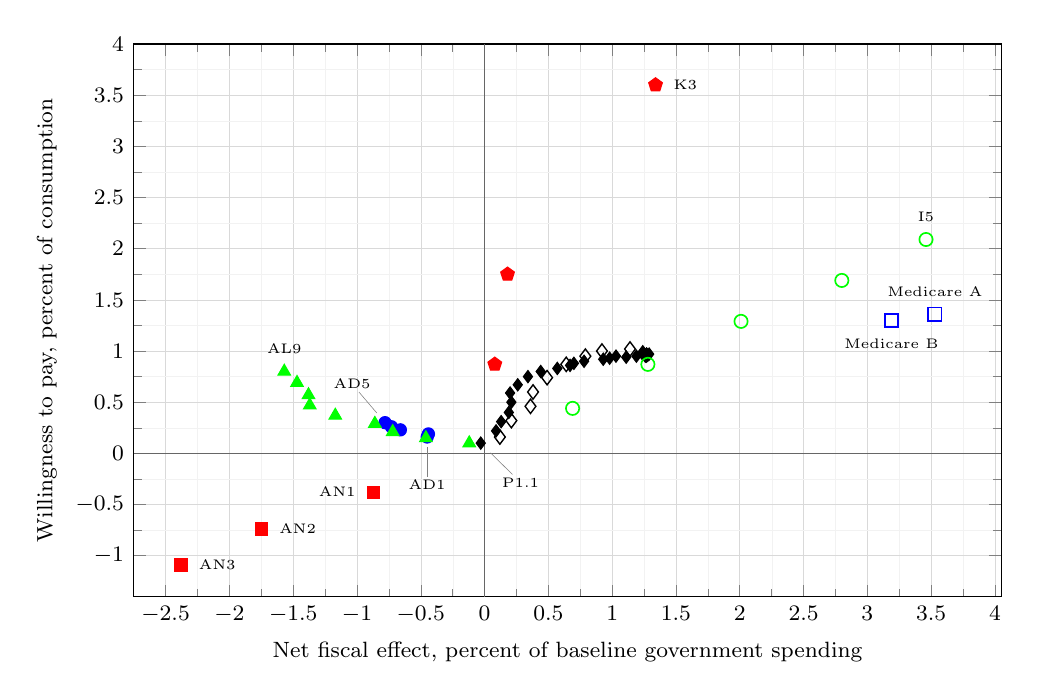
\begin{tikzpicture}
\begin{axis}[%
width=12.6cm,
height=8.6cm,
xlabel={Net fiscal effect, percent of baseline government spending},
ylabel={Willingness to pay, percent of consumption},
xmin=-2.75, xmax=4.05,
ymin=-1.4, ymax=4.0,
xtick={-2.5,-2,...,4},
ytick={-1,-0.5,...,4},
grid=both,
grid style={line width=0.2pt, draw=gray!30},
minor grid style={line width=0.1pt, draw=gray!10},
minor tick num=1,
axis background/.style={fill=white},
tick label style={font=\footnotesize},
label style={font=\footnotesize},
legend to name=legwtpnet,
legend columns=4,
legend style={draw=white!15!black, font=\scriptsize, /tikz/every even column/.append style={column sep=0.6em}},
legend cell align=left,
clip=false
]
% zero lines
\addplot [forget plot, black!60, line width=0.4pt] coordinates {(-2.75,0) (4.05,0)};
\addplot [forget plot, black!60, line width=0.4pt] coordinates {(0,-1.4) (0,4.0)};
% AN1-AN3                                                          % src: tables/welfare_age_dependence_mvpfv5.tex:108-110
\addplot [only marks, color=red, mark=square*, mark size=2.2pt] coordinates {(-0.87,-0.38) (-1.75,-0.74) (-2.38,-1.09)};
\addlegendentry{Higher NRA (AN1--AN3)}
% AD1-AD5                                                          % src: tables/welfare_age_dependence_mvpfv5.tex:112-116
\addplot [only marks, color=blue, mark=*, mark size=2.2pt] coordinates {(-0.45,0.16) (-0.44,0.19) (-0.66,0.23) (-0.73,0.26) (-0.78,0.3)};
\addlegendentry{Higher DRC (AD1--AD5)}
% AL1-AL9                                                          % src: tables/welfare_age_dependence_mvpfv5.tex:118-126
\addplot [only marks, color=green, mark=triangle*, mark size=2.6pt] coordinates {(-0.12,0.10) (-0.46,0.15) (-0.72,0.21) (-0.86,0.29) (-1.17,0.37) (-1.37,0.47) (-1.38,0.57) (-1.47,0.69) (-1.57,0.80)};
\addlegendentry{Symmetric adjustment (AL1--AL9)}
% P1.1-P1.9, P2.0-P2.9, P3.0-P3.9                                  % src: tables/welfare_progressivity_mvpfv7.tex:115-123, 126-135, 137-146
\addplot [only marks, color=black, mark=diamond*, mark size=2.2pt] coordinates {(-0.03,0.10) (0.09,0.22) (0.13,0.31) (0.19,0.40) (0.21,0.50) (0.20,0.59) (0.26,0.67) (0.34,0.75) (0.44,0.80) (0.57,0.83) (0.67,0.86) (0.70,0.88) (0.78,0.90) (0.93,0.92) (0.98,0.93) (1.03,0.95) (1.11,0.94) (1.19,0.95) (1.27,0.95) (1.26,0.95) (1.27,0.96) (1.28,0.96) (1.26,0.96) (1.27,0.96) (1.29,0.97) (1.27,0.97) (1.27,0.97) (1.25,0.97) (1.24,0.98)};
\addlegendentry{Progressivity (P1.1--P3.9)}
% L0-L9                                                            % src: tables/welfare_progressivity_mvpfv7.tex:149-158
\addplot [only marks, color=black, mark=diamond, mark size=2.6pt, line width=0.5pt] coordinates {(0.12,0.16) (0.21,0.32) (0.36,0.46) (0.38,0.60) (0.49,0.74) (0.64,0.87) (0.79,0.95) (0.92,1.00) (1.14,1.02) (1.24,0.98)};
\addlegendentry{Level (L0--L9)}
% Medicare Part A, Part B                                          % src: tables/welfare_medicare_mvpfv8.tex:113, 116-118
\addplot [only marks, color=blue, mark=square, mark size=2.4pt, line width=0.6pt] coordinates {(3.53,1.36) (3.19,1.30)};
\addlegendentry{Medicare Part A, Part B}
% I1-I5                                                            % src: tables/welfare_tax_mvpf_v8.tex:114-118
\addplot [only marks, color=green, mark=o, mark size=2.4pt, line width=0.6pt] coordinates {(0.69,0.44) (1.28,0.87) (2.01,1.29) (2.80,1.69) (3.46,2.09)};
\addlegendentry{Income tax (I1--I5)}
% K1-K3                                                            % src: tables/welfare_savings_mvpf_v3.tex:120, 122, 123
\addplot [only marks, color=red, mark=pentagon*, mark size=2.6pt] coordinates {(0.08,0.87) (0.18,1.75) (1.34,3.6)};
\addlegendentry{Saving subsidy (K1--K3)}
% point labels (selected rows)
\node [anchor=east, font=\tiny, xshift=-3pt] at (axis cs:-0.87,-0.38) {AN1};     % src: tables/welfare_age_dependence_mvpfv5.tex:108
\node [anchor=west, font=\tiny, xshift=3pt] at (axis cs:-1.75,-0.74) {AN2};     % src: tables/welfare_age_dependence_mvpfv5.tex:109
\node [anchor=west, font=\tiny, xshift=3pt] at (axis cs:-2.38,-1.09) {AN3};     % src: tables/welfare_age_dependence_mvpfv5.tex:110
\node [pin={[pin distance=11pt, font=\tiny, inner sep=1pt]270:AD1}] at (axis cs:-0.45,0.16) {};   % src: tables/welfare_age_dependence_mvpfv5.tex:112
\node [pin={[pin distance=8pt, font=\tiny, inner sep=1pt]110:AD5}] at (axis cs:-0.78,0.3) {};    % src: tables/welfare_age_dependence_mvpfv5.tex:116
\node [anchor=south, font=\tiny, yshift=3pt] at (axis cs:-1.57,0.80) {AL9};     % src: tables/welfare_age_dependence_mvpfv5.tex:126
\node [pin={[pin distance=9pt, font=\tiny, inner sep=1pt]300:P1.1}] at (axis cs:-0.03,0.10) {};  % src: tables/welfare_progressivity_mvpfv7.tex:115
\node [anchor=south, font=\tiny, yshift=3pt] at (axis cs:3.53,1.36) {Medicare A}; % src: tables/welfare_medicare_mvpfv8.tex:113
\node [anchor=north, font=\tiny, yshift=-3pt] at (axis cs:3.19,1.30) {Medicare B}; % src: tables/welfare_medicare_mvpfv8.tex:116-118
\node [anchor=south, font=\tiny, yshift=3pt] at (axis cs:3.46,2.09) {I5};       % src: tables/welfare_tax_mvpf_v8.tex:118
\node [anchor=west, font=\tiny, xshift=3pt] at (axis cs:1.34,3.6) {K3};         % src: tables/welfare_savings_mvpf_v3.tex:123
\end{axis}
\end{tikzpicture}

\vspace{2pt}
\pgfplotslegendfromname{legwtpnet}

\begin{minipage}{0.92\textwidth}
\vspace{4pt}
\scriptsize
\textit{Notes:} Each marker is one reform row of \autoref{tab:claiming}, \autoref{tab:other}, or \autoref{tab:progressivity_full}. The vertical axis is the WTP column, the consumption-equivalent welfare change in percent of consumption \eqref{eq:ce}; the horizontal axis is the Net column, the change in government spending on the cohort in percent of its baseline value, the Net base defined in \autoref{tab:conventions}. Rows with positive willingness to pay and a negative net fiscal effect (upper-left quadrant) are the rows with an infinite MVPF in the tables; the AN rows (lower-left quadrant) have negative willingness to pay and a negative net fiscal effect. Within a family the MVPF is proportional to the ratio WTP/Net by \eqref{eq:mvpfcolumns}, with a constant that differs across families, so rays from the origin order the MVPF within a family only. L9 and P3.9 are the same policy and plot at the same point; AD1 and AL2 nearly coincide. Source: authors' simulations of the estimated model.
% src: tables/welfare_age_dependence_mvpfv5.tex:108-126; tables/welfare_progressivity_mvpfv7.tex:115-158; tables/welfare_medicare_mvpfv8.tex:113,116-118; tables/welfare_tax_mvpf_v8.tex:114-118; tables/welfare_savings_mvpf_v3.tex:120-123
\end{minipage}
\end{figure}

